\documentclass{article}
\usepackage[UTF8]{ctex}
\usepackage{amsmath,mathtools,geometry,pgfplots,float,mathrsfs}
\pgfplotsset{compat=1.15}
\usetikzlibrary{arrows}
\geometry{scale=0.7}

\title{每日一题(14.1)}
\author{\kaishu 门宇翎}
\date{2022年4月12日}

\begin{document}
\maketitle
\textbf{1. }证明: 三角形的重心到一边中点的距离等于这条边上的中线之长的三分之一.
\begin{figure}[H]
	\flushright
	\definecolor{uuuuuu}{rgb}{0.26666666666666666,0.26666666666666666,0.26666666666666666}
	\begin{tikzpicture}[line cap=round,line join=round,>=triangle 45,x=3.0cm,y=3.0cm]
		\clip(-0.28957567281570085,-0.23558827532809026) rectangle (2.0105641679656974,1.4516732130139607);
		\draw [line width=1.2pt] (0.5334625068119092,1.30230611681789)-- (0.,0.);
		\draw [line width=1.2pt] (0.,0.)-- (1.7367968508018572,0.);
		\draw [line width=1.2pt] (1.7367968508018572,0.)-- (0.5334625068119092,1.30230611681789);
		\draw [line width=0.4pt] (0.5334625068119092,1.30230611681789)-- (0.8683984254009286,0.);
		\draw [line width=0.4pt] (1.1351296788068832,0.651153058408945)-- (0.,0.);
		\draw [line width=0.4pt] (0.2667312534059546,0.651153058408945)-- (1.7367968508018572,0.);
		\begin{scriptsize}
			\draw [fill=black] (0.,0.) circle (0.5pt);
			\draw[color=black] (-0.0495931854147524,-0.016835007966456525) node {$A$};
			\draw [fill=black] (0.5334625068119092,1.30230611681789) circle (0.5pt);
			\draw[color=black] (0.5115966312766962,1.3289129406127065) node {$B$};
			\draw [fill=black] (1.7367968508018572,0.) circle (0.5pt);
			\draw[color=black] (1.7761197379663092,0.005317221639784842) node {$C$};
			\draw [fill=uuuuuu] (1.1351296788068832,0.651153058408945) circle (0.5pt);
			\draw[color=uuuuuu] (1.1687794429285243,0.6717301289608794) node {$D$};
			\draw [fill=uuuuuu] (0.8683984254009286,0.) circle (0.5pt);
			\draw[color=uuuuuu] (0.8900305537166534,-0.04267927584040479) node {$E$};
			\draw [fill=uuuuuu] (0.2667312534059546,0.651153058408945) circle (0.5pt);
			\draw[color=uuuuuu] (0.22361764639555815,0.6643460524254655) node {$F$};
			\draw [fill=uuuuuu] (0.7567531192045889,0.43410203893929666) circle (0.5pt);
			\draw[color=uuuuuu] (0.773731348283886,0.5000503495125087) node {$G$};
		\end{scriptsize}
	\end{tikzpicture}
\end{figure}\par
\textbf{2$^\ast$. }如图, $D$为$BC$上一点, $E, F$分别是$\triangle ABD, \triangle ACD$的重心, 连接$EF$交$AD$于$G$. 求$\dfrac{DG}{GA}$.
\begin{figure}[H]
	\flushright
	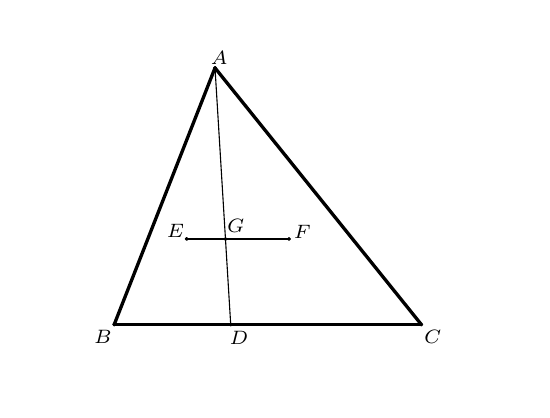
\begin{tikzpicture}[line cap=round,line join=round,>=triangle 45,x=3.0cm,y=3.0cm]
		\clip(-0.3663539802626259,-0.27732966665224645) rectangle (1.724682238629549,1.2565444136587105);
		\draw [line width=1.2pt] (0.42667975111943757,1.0861614245109785)-- (0.,0.);
		\draw [line width=1.2pt] (0.,0.)-- (1.3,0.);
		\draw [line width=1.2pt] (1.3,0.)-- (0.42667975111943757,1.0861614245109785);
		\draw [line width=0.4pt] (0.49313643993816175,0.)-- (0.42667975111943757,1.0861614245109785);
		\draw [line width=0.4pt] (0.30660539701919975,0.3620538081703262)-- (0.7399387303525331,0.36205380817032623);
		\begin{scriptsize}
			\draw [fill=black] (0.42667975111943757,1.0861614245109785) circle (0.5pt);
			\draw[color=black] (0.44421623942029587,1.1298403731078601) node {$A$};
			\draw [fill=black] (0.,0.) circle (0.5pt);
			\draw[color=black] (-0.047496129869758125,-0.05161187255834743) node {$B$};
			\draw [fill=black] (1.3,0.) circle (0.5pt);
			\draw[color=black] (1.348765615008484,-0.05329007177094147) node {$C$};
			\draw [fill=black] (0.49313643993816175,0.) circle (0.5pt);
			\draw[color=black] (0.5281262000499979,-0.05496827098353552) node {$D$};
			\draw [fill=black] (0.30660539701919975,0.3620538081703262) circle (0.5pt);
			\draw[color=black] (0.2596143260349514,0.3981455164168566) node {$E$};
			\draw [fill=black] (0.7399387303525331,0.36205380817032623) circle (0.5pt);
			\draw[color=black] (0.7966380740650445,0.3914327195664804) node {$F$};
			\draw [fill=black] (0.47098421033192034,0.36205380817032623) circle (0.5pt);
			\draw[color=black] (0.5147006063492456,0.4182839069679851) node {$G$};
		\end{scriptsize}
	\end{tikzpicture}
\end{figure}
\end{document}